\section{Zitate}

Im Literaturverzeichnis sollte zu jedem Zitat ein Eintrag mit dem entsprechenden Kürzel zu finden sein.

\subsection{Einzelner Autor}

Zur Überprüfung wird das Buch ``The Hitchhiker's Guide to the Galaxy``  von Douglas Adams aus dem Jahr 1979 hinzugezogen. Die folgende Zitierung sollte mit \texttt{[Ada79]}  abgekürzt dargestellt werden. \textit{Zitat} \cite{TestCitation001}.

\subsection{Zwei Autoren}

Zur Überprüfung wird das Buch ``Hard drive: Bill Gates and the making of the Microsoft empire`` von James Wallace und Jim Erickson aus dem Jahr 1992 hinzugezogen. Die folgende Zitierung sollte mit \texttt{[WE92]} abgekürzt dargestellt werden. \textit{Zitat} \cite{TestCitation002}.

\subsection{Drei Autoren}

Zur Überprüfung wird der Artikel ``Antioxidant activity of apple peels`` von Kelly Wolfe, Xianzhong Wu und Rui Hai Liu aus dem Jahr 2003 hinzugezogen. Die folgende Zitierung sollte mit \texttt{[WWL03]} abgekürzt dargestellt werden. \textit{Zitat} \cite{TestCitation003}.

\subsection{Viele Autoren}

Zur Überprüfung wird der Artikel ``Observation of top quark production in p p collisions with the Collider Detector at Fermilab`` von Fumio Abe, H. Akimoto, A. Akopian, M.G. Albrow, S.R. Amendolia, D. Amidei, J. Antos, C. Anway-Wiese, S. Aota, G. Apollinari und Weitere aus dem Jahr 1995 hinzugezogen. Die folgende Zitierung sollte mit \texttt{[AAA+95]} abgekürzt dargestellt werden. \textit{Zitat} \cite{TestCitation004}.

\newpage

\section{Tabellen}

Eine Tabelle sollte immer eine Über- oder Unterschrift erhalten und mit dieser im Tabellenverzeichnis wiederzufinden sein. Weiterhin muss ein Zitat angegeben werden, wenn es sich um hinzugezogene Daten handelt.

\subsection{Simple Tabelle}

\begin{table}[H]
\centering
\begin{tabular}{|l|l|} 
\hline
Spezifische Wärmekapazität (J/(mol K)) & Temperatur (°C)  \\ 
\hline
12,2                                   & -200             \\ 
\hline
15,0                                   & -180             \\ 
\hline
17,3                                   & -160             \\ 
\hline
19,8                                   & -140             \\ 
\hline
24,8                                   & -100             \\ 
\hline
29,6                                   & -60              \\
\hline
\end{tabular}
\caption{Spezifische Wärmekapazität von Wasser \cite{TestCitation020}}
\end{table}

\subsection{Komplexere Tabelle}

\newcommand{\tabtitel}[1]{\multicolumn{2}{l|}{\textbf{#1}}}

\begin{table}[H]
\centering
\begin{tabular}{|l|l|l|l|l|} 
\hline
           & \tabtitel{Ostdeutschland} & \tabtitel{Westdeutschland}  \\ 
\hline
Geschlecht & Frauen & Männer           & Frauen & Männer                       \\ 
\hline
weiblich   & 100\%  & 0\%              & 100\%  & 0\%                          \\ 
\hline
männlich   & 0\%    & 100\%            & 0\%    & 100\%                        \\
\hline
\end{tabular}
\caption{Absurder Vergleich von Ost- und Westdeutschland}
\end{table}

\newpage

\section{Grafiken, Bilder, etc.}

Eine Tabelle sollte immer eine Über- oder Unterschrift erhalten und mit dieser im Tabellenverzeichnis wiederzufinden sein.

\subsection{Simple Grafik}

\begin{figure}[H]
	\centering
	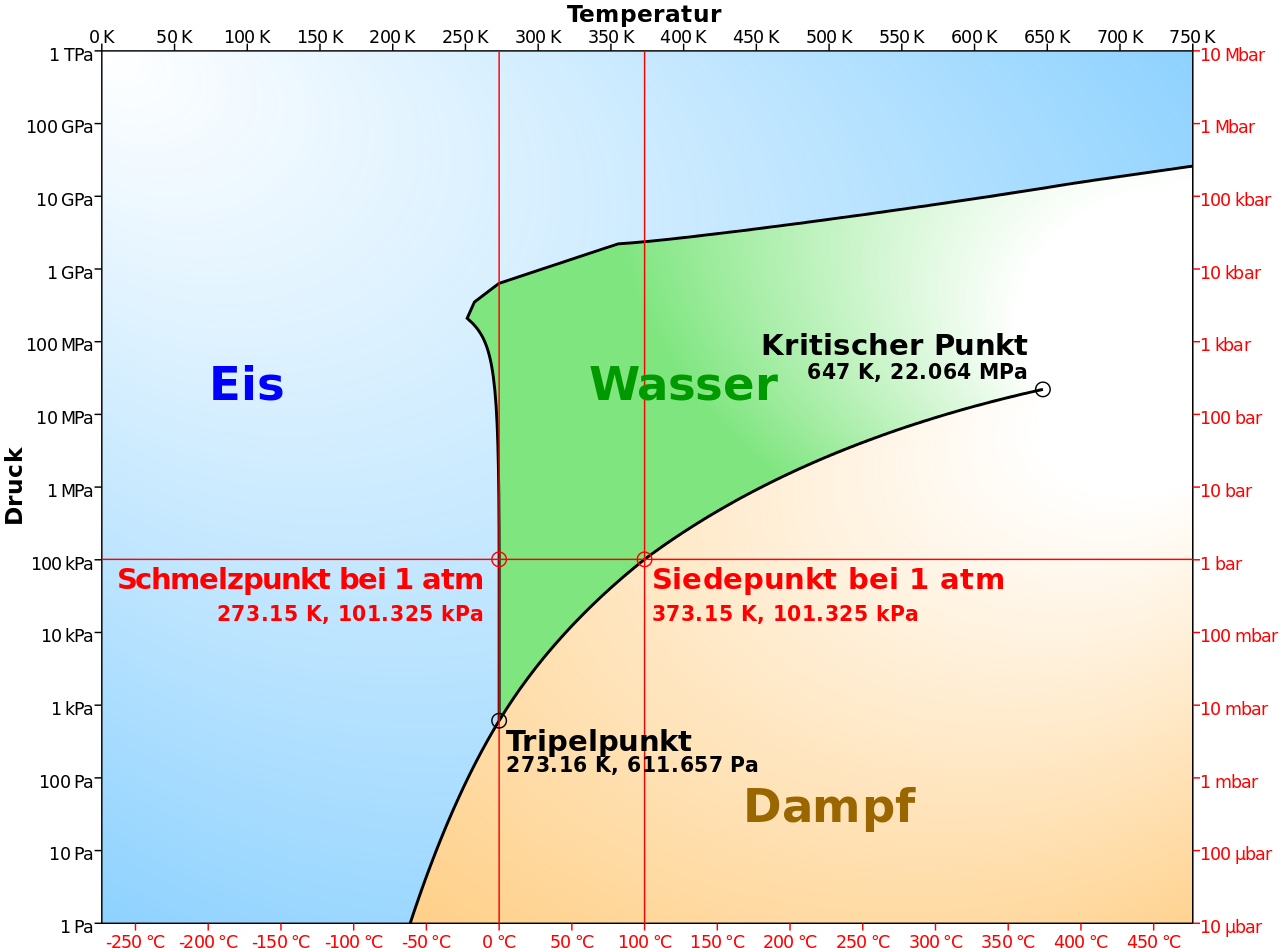
\includegraphics[width=\linewidth]{content/xx_test/Phase_diagram_of_water_simplified.svg.png}
	\caption{Vereinfachtes Phasendiagramm von Wasser \cite{TestCitation020}}
\end{figure}

\newpage

\subsection{Innerhalb eines Textes (Floating)}

\begin{wrapfigure}[14]{r}{0.33\textwidth}
	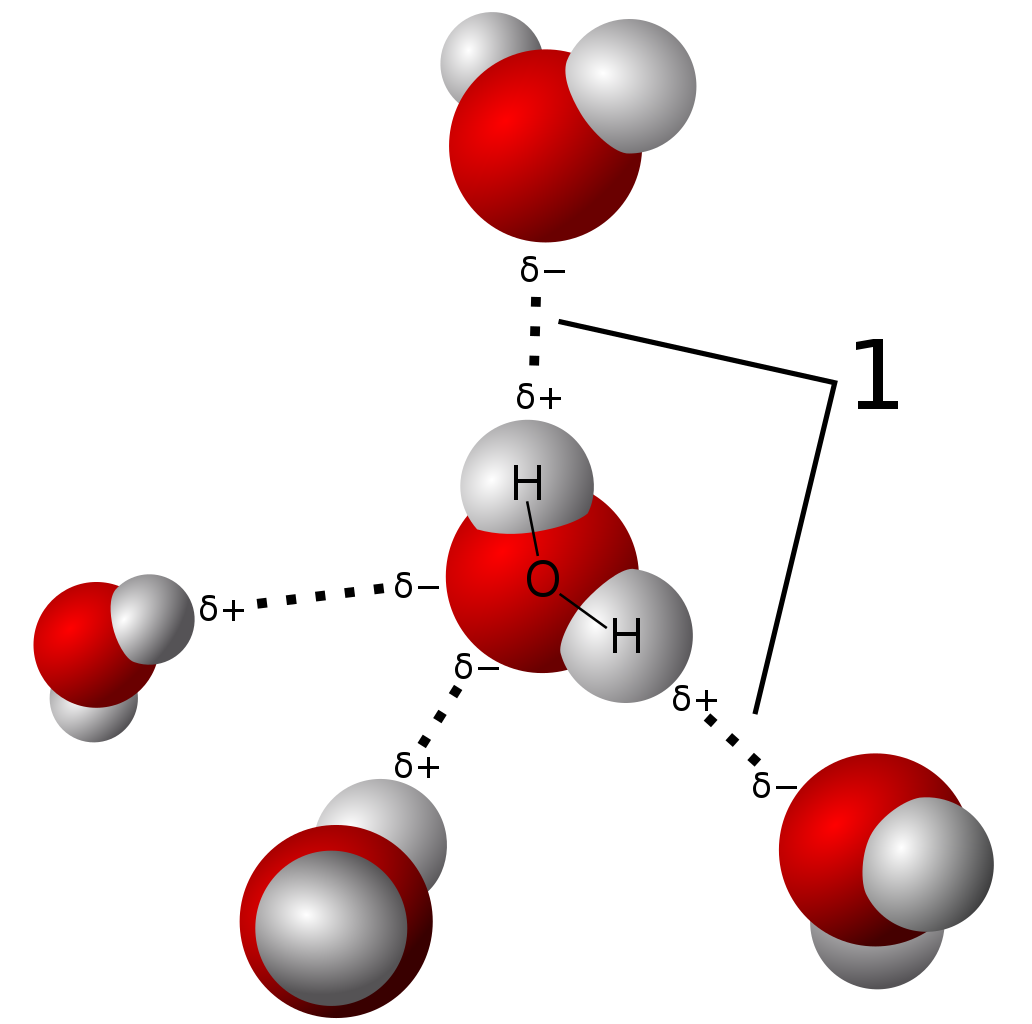
\includegraphics[width=\linewidth]{content/xx_test/1032px-3D_model_hydrogen_bonds_in_water.svg.png}
	\caption{Verkettung der Wassermoleküle \cite{TestCitation021}}
\end{wrapfigure}

Lorem ipsum dolor sit amet, consectetur adipiscing elit. Praesent eu risus a erat auctor bibendum. Morbi eget aliquet nisl. Aenean vestibulum elit sed arcu condimentum euismod. Nunc quis ipsum sed augue maximus molestie. Pellentesque condimentum elit vitae justo tincidunt elementum. Aliquam erat volutpat. Vestibulum feugiat auctor fringilla.

Cras non arcu ante. Donec faucibus lectus risus, ac sagittis risus malesuada pretium. Cras elementum quis turpis accumsan faucibus. Vestibulum vitae volutpat nisl, et sodales nunc. Etiam egestas at magna a commodo. Mauris sagittis suscipit tempus. Duis rhoncus nec ligula eget viverra. Maecenas eu nisl orci. Proin dignissim laoreet libero in interdum. Lorem ipsum dolor sit amet, consectetur adipiscing elit.

Sed fringilla lectus non elit convallis, non eleifend sem porta. Proin aliquet urna ultrices metus blandit ornare. Duis nec ultricies ligula, quis volutpat ante. Suspendisse non lacus mauris.

\begin{wrapfigure}[14]{o}{0.45\textwidth}
	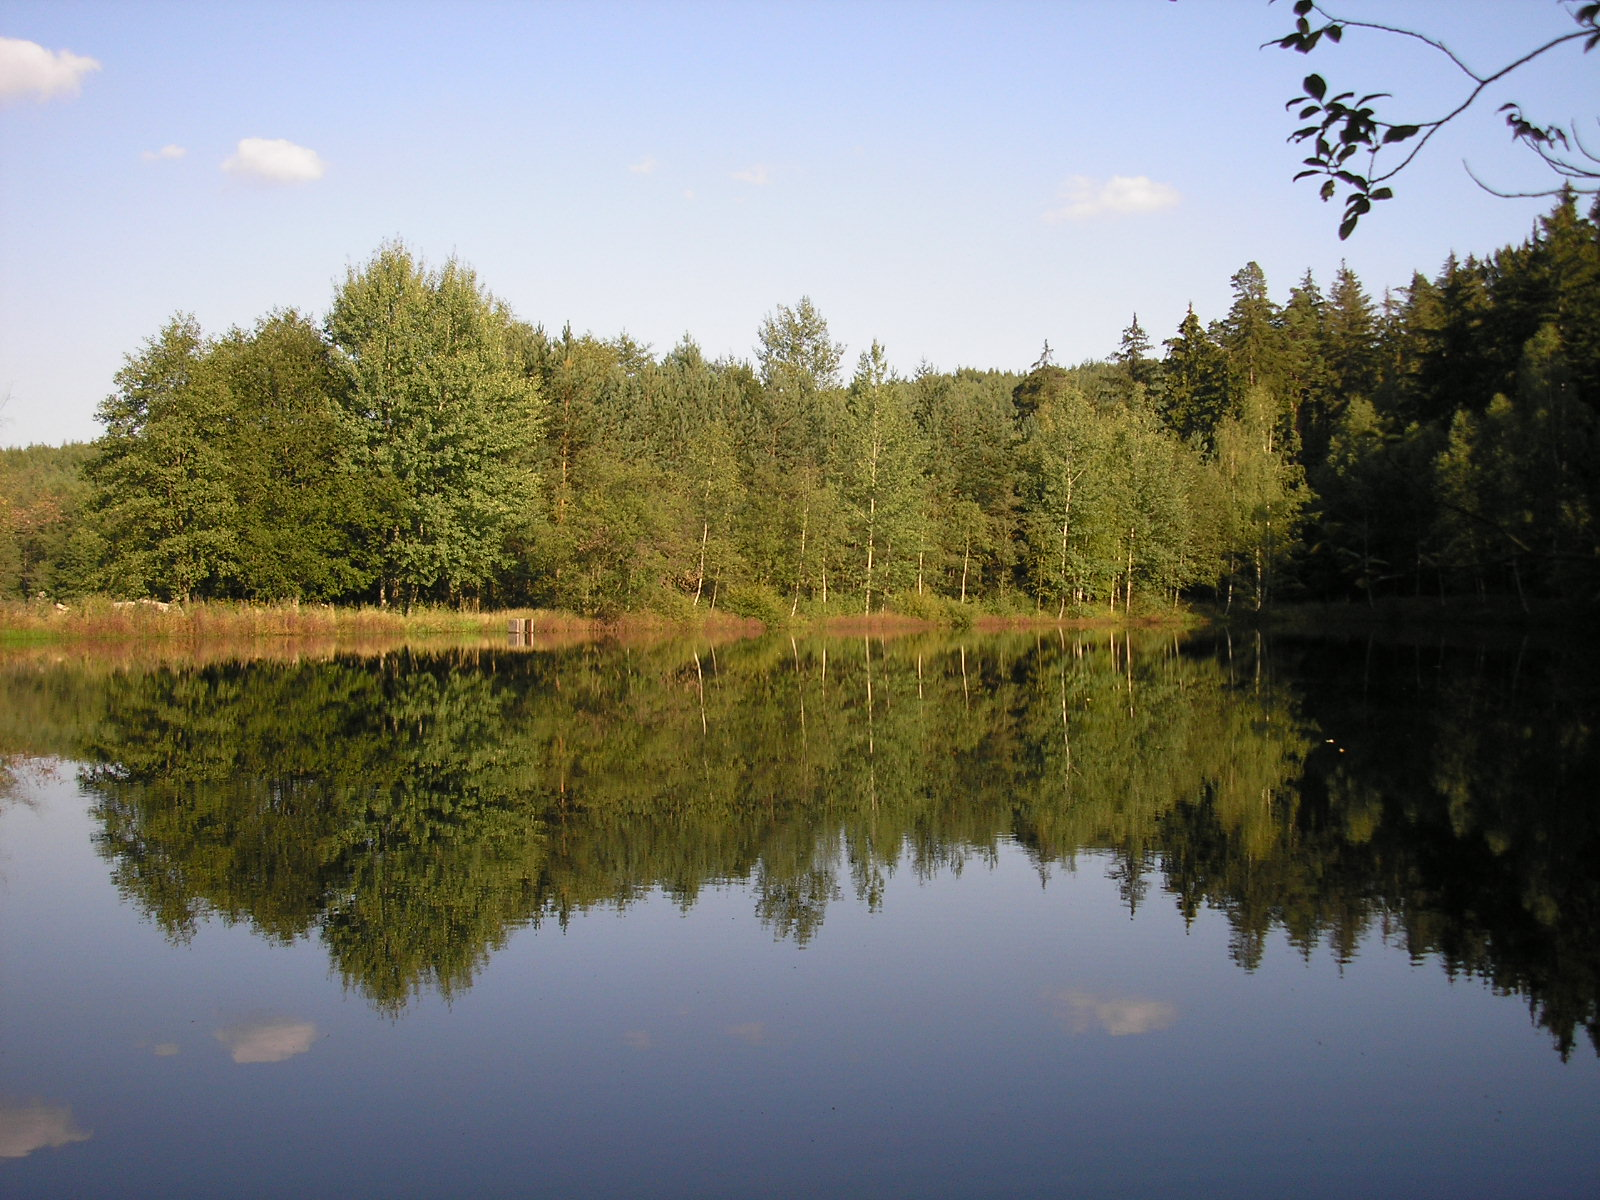
\includegraphics[width=\linewidth]{content/xx_test/Kleiner_Streichteich_Ilmenau.JPG}
	\caption{Spiegelung an der Wasseroberfläche \cite{TestCitation022}}
\end{wrapfigure}

Nullam quam diam, mattis non bibendum vel, iaculis sed leo. Phasellus condimentum auctor ante in mollis. Nullam rhoncus enim ac metus fermentum aliquam. Phasellus orci metus, tristique ac odio sed, fermentum faucibus mauris. Praesent vehicula risus aliquam nibh sodales, ac aliquam ante posuere. Praesent at semper sapien. In posuere augue vel tortor posuere rhoncus. Duis eget quam tempus diam posuere fringilla ut vitae lacus. Sed sagittis fringilla diam.

Suspendisse potenti. Ut pellentesque malesuada dolor vitae porta. Aliquam erat volutpat. Proin convallis mauris neque. Etiam et accumsan ex. Class aptent taciti sociosqu ad litora torquent per conubia nostra, per inceptos himenaeos. Suspendisse potenti. Cras ac magna enim. Praesent ultrices lacinia sem nec placerat. Sed tristique non sapien quis efficitur. Ut sit amet egestas metus. Mauris nec erat sodales, semper dolor eu, egestas justo. Ut sit amet urna ligula.

\section{Quellcode}

Der jeweilige Quellcode sollte mit Syntax-Highlighting versehen sein und im Quellcodeverzeichnis aufzufinden sein.

\subsection{Darstellung eines JavaScript Quellcodes (inline)}

\begin{lstlisting}[
  language = JavaScript,
     style = ES6,
   caption = Beispiel eines JavaScript Quellcodes (inline),
captionpos = b,
     label = lst:javascript-inline-example,
]
var fetch = require("node-fetch")

async function getCountries() {
  let res = await fetch("https://restcountries.eu/rest/v2/name/Indonesia?fullText=true")
  let json = await res.json()
  let code = json[0].alpha2Code
  let res2 = await fetch("http://country.io/phone.json")
  let json2 = await res2.json()
  console.log(json2[code])
}

getCountries()
\end{lstlisting}

\subsection{Darstellung eines JavaScript Quellcodes (importiert)}

\lstinputlisting[
  language = JavaScript,
     style = ES6,
   caption = Beispiel eines JavaScript Quellcodes (importiert),
captionpos = b,
     label = lst:javascript-import-example,
]{content/xx_test/import-example_javascript.js}

\subsection{Darstellung eines Java Quellcodes (inline)}

\begin{lstlisting}[
   caption = Beispiel eines Java Quellcodes (inline),
     label = lst:java-inline-example,
  language = java, 
     style = java-eclipse,
basicstyle = {\footnotesize\fontfamily{pcr}\selectfont}
]
	/*
	 * Main-Methode
	 */
	§§@LineAnnotation
	public class Main {
	  public static void main(%%@InlineAnnotation%% String[] args) {
	    System.out.println("Hallo Welt");
	  }
	}
\end{lstlisting}

\subsection{Darstellung eines Java Quellcodes (importiert)}

\lstinputlisting[
   caption = Beispiel eines Java Quellcodes (importiert),
     label = lst:java-import-example,
  language = java,
     style = java-eclipse,
basicstyle = {\footnotesize\fontfamily{pcr}\selectfont}
]{content/xx_test/import-example_java.js}